\section{Le Perceptron}
\fancyhead[R]{\textit{\nouppercase{\leftmark}}}

\subsection{Modèle du perceptron}

Le perceptron est un des algorithmes de base du machine learning. Son invention remonte aux années 70, mais a été abandonné alors, 
son exécution étant trop coûteuse pour les performances des ordinateurs de l’époque. Ce n’est que récemment qu’il a pu resurgir, grâce 
à l’amélioration des processeurs et des cartes graphiques, particulièrement adaptés aux calculs matriciels.

Le modèle du neurone est le suivant : 

\begin{figure}[h]
 \centering
 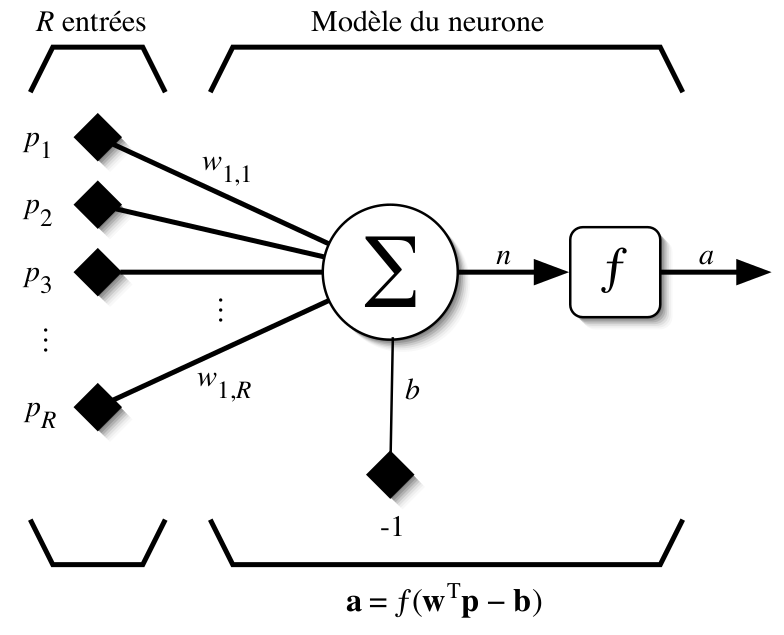
\includegraphics[width=0.5\textwidth]{img/neurone.png}
 \caption{Modèle d'un neurone artificiel}
\end{figure}

Le neurone est composé de différents élements : 
\begin{itemize}
 \item $p_1$, $p_2$, ..., $p_R$ constituent les $R$ variables d'entrées du perceptron. Le nombre d'entrée est souvent imposé par le système lui-même.
 \item $w_{1,1}$, $w_{1,2}$, ..., $w_{1,R}$ sont les poids associés respectivement à chaque entrée. Il mesure l'importance accordée à chaque entrée. Un poids
 plus important signifie que l'entrée associée est plus pertinente pour ce neurone que les autres.
 \item Le biais $b$
 \item Le niveau d'activation $n$
 \item La fonction d'activation $f$
 \item La sortie $a$
\end{itemize}

Ainsi, on associe les entrées et les poids par un produit scalaire, pour en sortir une valeur qui caractérise l'entrée, le niveau d'activation.
On ajoute un biais pour régler l'importance accordée au niveau d'activation. On peut utiliser une notation matricielle pour simplifier les calculs.
On pose alors $w_1 = 
\begin{pmatrix}
  w_{1,1} & w_{1,2} & \ldots & w_{1,R}\\
\end{pmatrix}^T $ 
et
$ p = 
\begin{pmatrix}
 p_1 & p_2 & \ldots & p_R \\
\end{pmatrix}^T $ 
les vecteurs colonnes représentant respectivement l'entrée et les poids du neurone. On a alors :

\begin{equation} 
n = \sum_{i=1}^{R} w_{1,j} p_j - b = \mathbf{w_1}^T \mathbf{p} - b
\end{equation}

On cherche alors à discriminer les différentes possibilités pour le niveau d'activation. C'est le rôle de la fonction d'activation. Si l'on souhaite séparer
le cas d'un $n$ supérieur ou non à un seuil donné alors on utilise la fonction seuil $ f : x \mapsto \mathds{1}_{n \geq 0} $. On remarquera qu'il n'est 
pas nécessaire de changer le seuil de la fonction car c'est le rôle incarné par le biais. Néanmoins, d'autres fonctions peuvent être utilisées à la place
du seuil telles que la sigmoide ($\sigma : x \mapsto \frac{1}{1+e^{-x}}$) ou encore $\tanh$. On préfère généralement des fonctions différentiables pour
permettre au réseau d'apprendre sur les données fournies.

On a alors : 
\begin{equation}
 a = f(\mathbf{w_1}^T \mathbf{p} - b)
\end{equation}

Si on revient au cas de la fonction seuil, on remarquera qu'elle permet de séparer le plan en deux espaces : l'un où la sortie est nulle, l'autre où
la sortie est égale à 1. Puisque le niveau d'activation résulte d'un produit matriciel, alors cela définit l'équation d'un hyperplan, donc la séparation
est linéaire.

\begin{figure}[h]
 \centering
 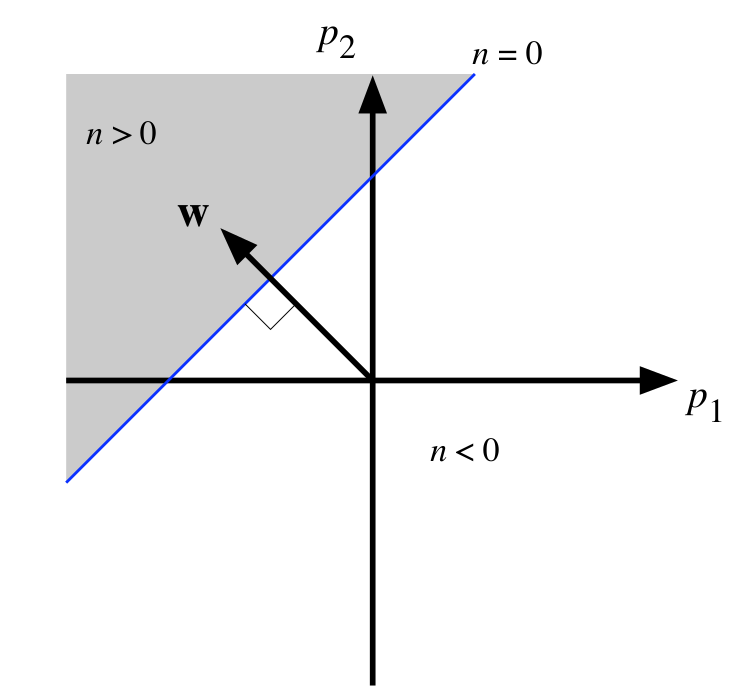
\includegraphics[width=0.5\textwidth]{img/separation_lineaire_du_plan.png}
 \caption{Domaine de séparation du neurone}
\end{figure}

Ce neurone n'est capable de traiter les données qui peuvent être séparées linéairement (par un hyperplan). Pour des jeux de données plus complexes,
on a parfois besoin de définir des ensembles plus élaborées.
Pour cela on utilise plusieurs neurones sur une même couche. Chacun d'entre eux reçoit la même entrée mais possède ses propres poids et son propre biais.
Ainsi, chaque neurone de la couche définit un hyperplan de séparation des données. On peut alors à nouveau représenter le modèle de manière matricielle.
Un vecteur de sortie définit les différentes valeurs des neurones, une matrice de poids définit les poids pour chaque neurone (à chaque neurone est associé
une ligne de la matrice). De la même manière, on retrouve un vecteur de biais (qui sont essentiellement des poids dont l'entrée est constante à $-1$), et 
un vecteur de niveaux d'activation. Finalement, on retrouve ce modèle : 

\begin{figure}[h]
 \centering
 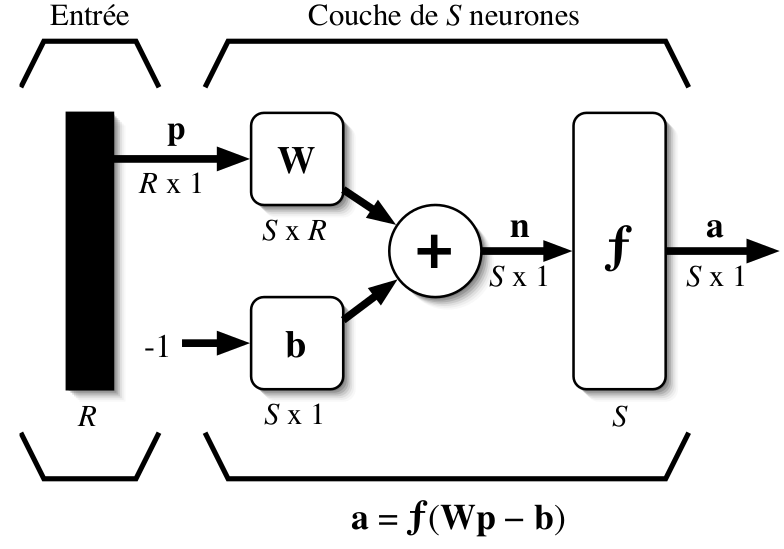
\includegraphics[width=0.55\textwidth]{img/couche.png}
 \caption{Représentation matricielle d'une couche de S neurones recevant R entrées}
\end{figure}

Pour pouvoir définir des ensembles de solution plus complexes, on ajoute d'autres couches de neurone. Chaque couche prend en entrée le vecteur de sortie
de la couche qui la précède. Cela permet donc de traiter les différents hyperplans de la première couche, et de les lier (par exemple pour en faire
l'intersection). Ainsi, avec deux couches, le réseau peut représenter n'importe quel ensemble convexe. Une troisième couche permet de représenter des
ensembles non convexes.

\begin{figure}[h]
 \centering
 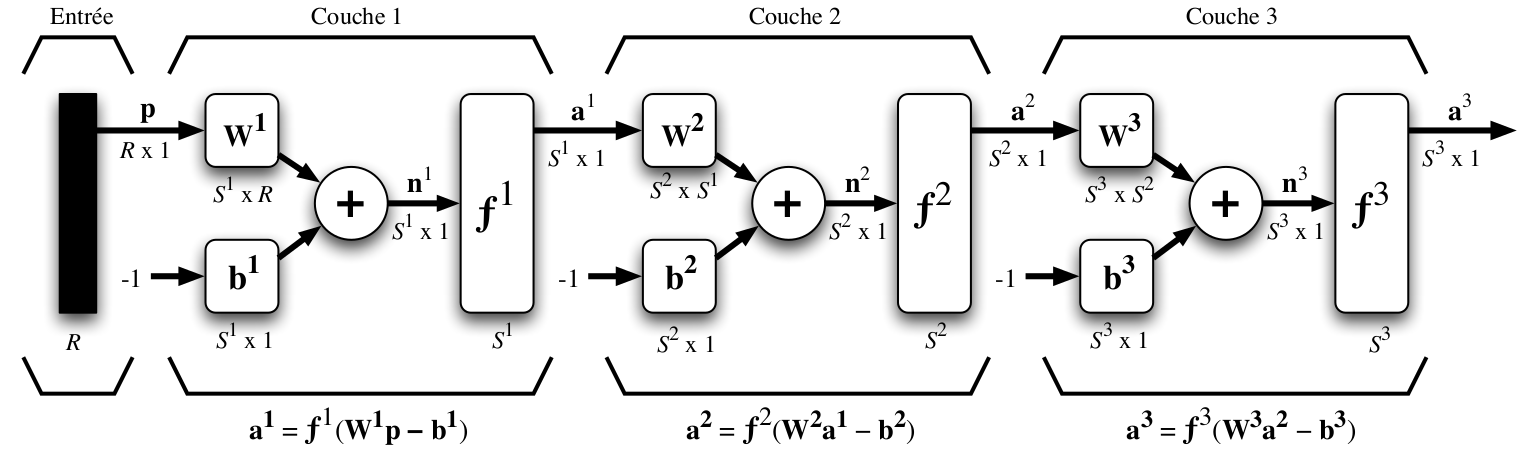
\includegraphics[width=\textwidth]{img/modele_perceptron_multicouches.png}
 \caption{Modèle du perceptron multicouches}
\end{figure}


\subsection{Apprentissage}

L'intérêt du modèle serait limité s'il devait être calculé manuellement. L'objectif est d'avoir un algorithme qui trouve lui-même les paramètres du réseau
(poids et biais) pour s'adapter à un jeu de données collectées au préalable. Il existe plusieurs méthodes pour réaliser l'apprentissage. Dans le cas du 
perceptron on utilise souvent un apprentissage supervisé. Cela signifie qu'avec les données collectées, il y ait également la ``bonne'' réponse pour que 
le réseau puisse apprendre en conséquence. D'autres méthodes comme l'apprentissage non supervisé existent, cette dernière reposant uniquement sur les jeux 
d'entrées, le réseau devant alors les discriminer lui-même sans connaître la ``bonne'' réponse.

Pour réaliser cela, on présente à notre réseau une entrée et, puisqu'on dispose de la sortie attendue, on peut mesurer à quel point le réseau s'est trompé.
C'est le rôle de la fonction d'erreur. Plus celle-ci est importante, moins le réseau est adapté pour cette donnée. Il existe différentes fonctions
d'erreur. Une des plus utilisées est la somme des carrés des écarts entre la valeur attendue et la valeur calculée : 

\begin{equation}
\displaystyle F(\mathbf{x}) = \mathbf{e(x)}^T\mathbf{e(x)} 
\end{equation}

où $\displaystyle \mathbf{e(x)} = \mathbf{d(x)} - \mathbf{a(x)} $ ,
$\mathbf{d(x)}$ la valeur attendue et $\mathbf{a(x)}$ la valeur calculée


L'apprentissage consiste donc en la minimisation de cette fonction de coût $F$. À chaque calcul d'erreur, on modifie les différents poids du réseau.
À une couche $k$ donnée, le poids entre l'entrée $j$ et le neurone $i$ est modifié de la manière suivante : 
\begin{equation}
 \Delta w^k_{i,j}(t) = - \eta \frac{\partial F}{\partial w^k_{i,j}}
\end{equation}
 
En se plaçant dans l'espace des poids (cela inclut les biais qui sont des poids particuliers), cela revient à chercher la direction dans laquelle l'erreur
est diminuée de la manière la plus significative. Le facteur $\eta$ est le taux d'apprentissage (Learning Rate en anglais). Il représente le pas de
chaque itération vers le minimum de la fonction de coût. C'est un paramètre du réseau que nous devons choisir en amont de l'apprentissage.

Marc \textsc{Paruzeau} démontre en 2004 les formules de rétropropagation que nous avons utilisées. Pour cela il introduit un paramètre % pas vraiment un paramère quand pensez-vous ? je ne trouve aps le mot juste
intermédiaire. Les sensibilités sont définies ainsi :
\begin{equation}
 \mathbf{s}^k = \frac{\partial F}{\partial \mathbf{n}^k}
\end{equation}

On note également l'utilisation du raccourci suivant : 

\begin{equation}
  \displaystyle
 \mathbf{\dot F}^k(\mathbf{n}^k) =
 \begin{bmatrix}
  \dot f ^k(n^k_1) & 0 & \ldots & 0\\
  0 & \dot f^k(n^k_2) & 0 & 0\\
  \vdots & \vdots & \ddots & \vdots \\
  0 & 0 & \ldots & \dot f^k(n^k_{S^k})\\
 \end{bmatrix}
 \text{où $S^k$ est le nombre de neurone de la couche $k$}
\end{equation}

Pour un réseau de $M$ couches, la rétropropagation se déroule de la manière suivante.
\begin{itemize}
 \item On propage notre entrée $\mathbf{p}$ dans le réseau
 \begin{equation}
   \mathbf{a}^k = \mathbf{f}^k(\mathbf{W}^k\mathbf{a}^{k-1} - \mathbf{b}^k) \text{, pour $k \in [1,M]$ et $\mathbf{a}^0 = \mathbf{p}$}
 \end{equation}
 
 \item On calcule les sensibilités 
 \begin{align}
  \mathbf{s}^M &= -2\mathbf{\dot F}^M(\mathbf{n}^M)\mathbf{e} \\
  \mathbf{s}^k &= \mathbf{\dot F}^k(\mathbf{n}^k)(\mathbf{W}^{k+1})^T \mathbf{s}^{k+1} \text{, pour $k \in [1,M-1]$}
 \end{align}
 
 \item On calcule les changements de poids
 \begin{align}
  \Delta \mathbf{W}^k &= - \eta \mathbf{s}^k(\mathbf{a}^{k-1})^T \text{, pour $k \in [1,M]$} \\
  \Delta \mathbf{b}^k &= \eta \mathbf{s}^k \text{, pour $k \in [1,M]$}
 \end{align}



\end{itemize}







\newpage


\subsection{Implémentation}

Afin de pouvoir comprendre en détail le fonctionnement du perceptron, nous avons commencé dans un premier temps à implémenter un version 
de celui-çi chacun de notre côté. Cela nous a permis de commencer  à réfléchir à l’architecture du code que nous voulions, et de pouvoir 
comparer les performances des différentes implémentations. 

Nous avons testé dans un premier temps les résultats de nos perceptrons sur la fonction XOR. Cette fonction est un bon départ pour pouvoir 
avoir un code fonctionnel, car il s’agit d’une fonction ne pouvant pas être répliquée par une fonction linéaire : il faut au moins une couche 
cachée afin de pouvoir l’implémenter grâce à un perceptron. 
Cette prémière étape nous a permis de comparer les résultats et les performances de nos algorithmes, et de pouvoir choisir l’implémentation 
du perceptron que nous avons utilisé par la suite.


\subsection{Résultats}


